% vim: set spell spelllang=es syntax=tex :

\section{Descripción de un sistema de visión global para fútbol de robots físicos
orientado al uso educativo}

\sectionmark{Descripción del sistema de visión global para fútbol de robots...}

\label{descripcionSistemaBase}

El principal objetivo del sistema descripto en \cite{torres2014} es su
utilización como herramienta didáctica para la introducción a la visión por
computadora. El sistema define un framework de visión por computadora capaz de
adaptarse a distintos dominios, pero en el trabajo se ofrece una solución
específica para el fútbol de robots de la liga de tamaño pequeño.

El sistema está basado en pilas de plugins y utiliza múltiples hilos para
aprovechar hasta cuatro núcleos (para el fútbol de robots); pero si la
plataforma posee más núcleos, no serán utilizados. Cada uno de los hilos tiene
una responsabilidad diferente. El framework general tiene tres componentes
principales:

\begin{description}

	\item[Hilo principal:] es el hilo encargado de la interfaz gráfica de
		usuario.

	\item[Hilo de captura de cuadros:] es el hilo encargado de la captura o
		generación de los cuadros a partir de una cámara o archivo. El
		hilo de captura está desacoplado de los hilos procesamiento de
		cuadros.

	\item[Hilos de procesamiento de cuadros:] cada uno de estos hilos tiene
		una pila de plugins creada con el objetivo de reconocer un tipo
		específico de objeto en un cuadro. En el caso del fútbol de
		robots habrá uno de estos hilos con una pila de plugins diseñada
		para encontrar los robots, y otro con una pila de plugins creada
		con el fin de encontrar la pelota. Para reconocer los objetos,
		el cuadro es procesado por cada uno de los plugins de la pila en
		forma secuencial y en un orden especifico. Existen mecanismos de
		control para asegurar que una vez que un cuadro haya sido procesado por
		uno de los hilos de procesamiento, será procesado por los
		restantes. Además, se asegura que ningún cuadro sea procesado
		dos veces por el mismo hilo de procesamiento.

\end{description}

En la implementación de la solución específica para el fútbol de robots de la
\emph{SSL}, se crean dos hilos de procesamiento de cuadros, uno para la búsqueda
de los robots y el otro para la búsqueda de la pelota. Las primeras etapas de
procesamiento son iguales en ambos. Los primeros plugins son los de
\emph{conversión de color}, \emph{segmentación de color} y \emph{morfología}. El
hilo de procesamiento que busca la pelota continúa con el plugin de
\emph{búsqueda de pelota}, mientras que aquél encargado de la búsqueda de robots
continúa con los plugins de \emph{detección de regiones principales} y
\emph{detección de regiones secundarias}. Ambos terminan con el plugin de
\emph{difusión}. En la figura \ref{pilasPlugins} se muestran ambas pilas y los
plugins que las componen. Como ambas pilas ejecutan los primeros tres plugins
sobre el mismo cuadro, se plantea la posibilidad de ejecutarlos una sola vez por
cuadro.

\begin{figure}[!htb]

	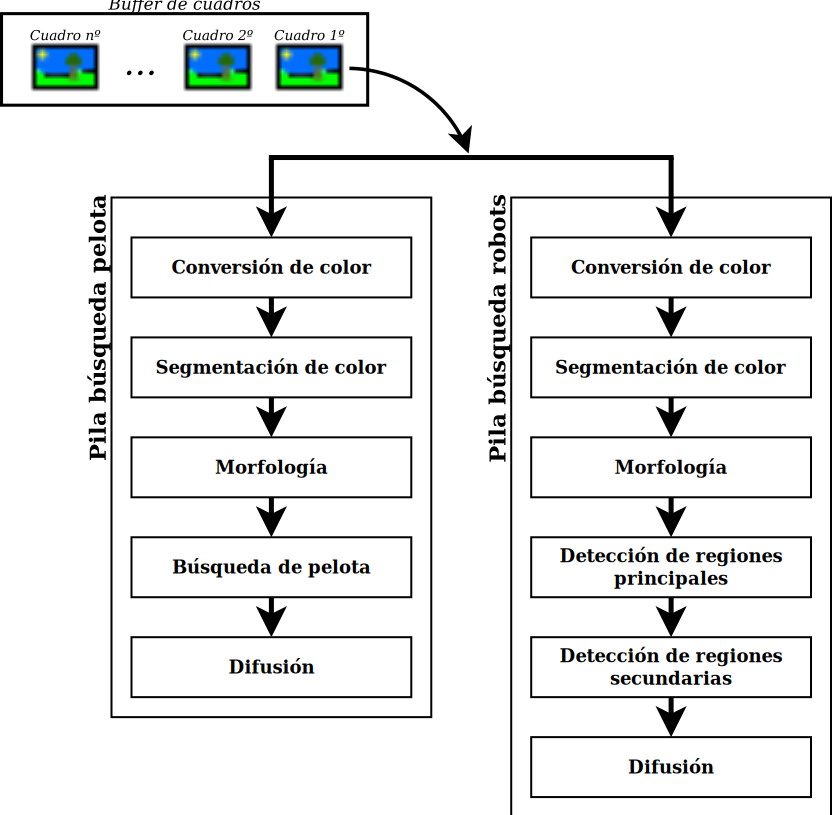
\includegraphics[width=\textwidth]{img/pilas.pdf}

	\caption{Pilas de plugins del sistema propuesto en \cite{torres2014}.}

	\label{pilasPlugins}

\end{figure}


De acuerdo a su función, los plugins pueden ser agrupados por las etapas de la
visión por computadora que implementan:

\begin{description}

	\item[Adquisición de la imagen:] Esta etapa está a cargo del hilo de
		captura de cuadros.

	\item[Preprocesamiento:] plugins de conversión de color, de segmentación
		de color y de morfología.

	\item[Extracción de características, Detección y Segmentación:] plugins
		de detección de regiones principales.

	\item[Procesamiento de alto nivel:] plugins de detección de pelota y de
		detección de regiones secundarias.

	\item[Toma de decisiones:] Dado que el sistema de visión para fútbol de
		robots no realiza toma de decisiones, el estado de la cancha es
		comunicado a las computadoras de los equipos a través del plugin
		de difusión.

\end{description}

El tiempo de generación de cuadros es fijo (o a demanda), mientras que el de
procesamiento es variable, pudiendo ser mayor o menor que el tiempo de
generación. Por ello, cuando se genera un nuevo cuadro, éste se coloca en un
buffer. Si la capacidad de procesamiento es insuficiente, y no hay más espacio
en el buffer para almacenar un nuevo cuadro, se descarta el cuadro más viejo.
Esta estrategia da mayor prioridad a la información más actual.

